% variational.tex
%
% Predrag created file				jul 9 2006
% $Author$ $Date$


\section{\descent}

%     Let $A[\pSpace]$ be an action functional defined loops $\Loop$
% emebedded in the state space manifold $\pS$, invariant
% under a diffeomorphism $g : \pS \to\pS$. Our aim is to determine
% the critical points of the action functional
% $ %\beq
% 	A[\pSpace]
%   % =\int_0^T  dt L(\pSpace,\dot\pSpace, t)
% $ % \label{McC2}
%   % \eeq
% defined on $\Lambda_g^1(\pS)$, a Sobolev space of paths in $\pS$ satisfying 
% \refeq{McC1}.
% \PC{define Sobolev space as adding a vector space?}

The strategy
is to minimize an action functional defined on a space of paths $\pSpace$ in the
configuration space $\pS$ which satisfy the property
\beq
                               \pSpace (t + T ) = g \cdot \pSpace (t)                       
\label{McC1}
\eeq
for a fixed {\em relative period} $T$ and some fixed diffeomorphism $g$ of $\pS$, 
sometimes referred to as a {\em phase}, that leaves the 
action functional invariant. If $g^k=1$ is of finite order
$k$, then the corresponding orbit is periodic with period $k T$. 

% %%%%%%%%%%%%%%%%%%%%%%%%%%%%%%%%%%%%%%%%%%%%%%%%%%%%%%%%%%%%%%%%
% \begin{figure}[t] %[h]
% \centering
% (c) 
\includegraphics[width=2.5cm]{figs/path.eps}
% \hspace{0.1in}
% (b) 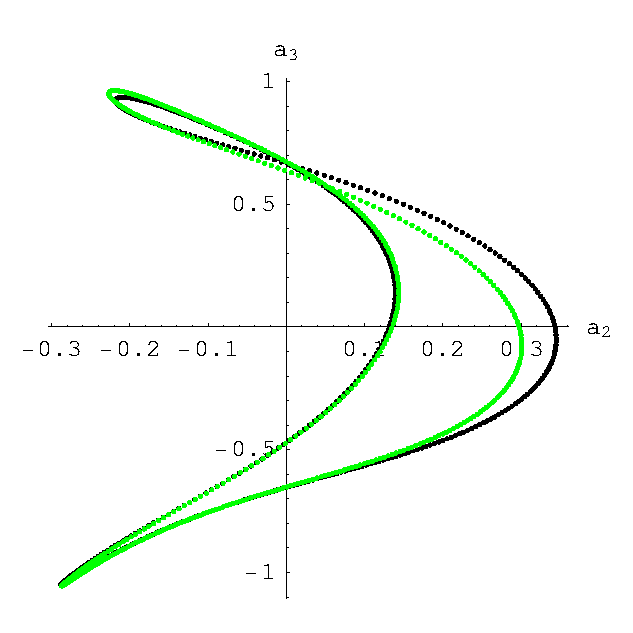
\includegraphics[width=3.5cm]{figs/loop.eps}
% \hspace{0.1in}
% (c) 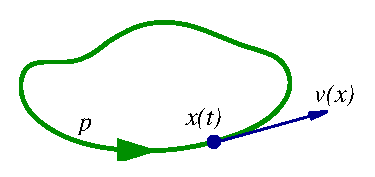
\includegraphics[width=4.0cm]{figs/porbit.eps}
% \caption{
%  (a) A continuous path; (b) a loop $\Loop$ with its tangent velocity vector $\lVeloc$;
%  (c) a periodic orbit $p$ defined by the vector field $\pVeloc(\pSpace)$.
%         }
% \label{f:loops}
% \end{figure}
% %%%%%%%%%%%%%%%%%%%%%%%%%%%%%%%%%%%%%%%%%%%%%%%%%%%%%%%%%%%%%%%%%%
% 
%     In order to set the notation, we shall distinguish between (see \reffig{f:loops}):
% 
% \medskip
% \noindent
%  {\bf closed path:}
%  any closed (not necessarily differentiable) continuous curve 
% $J \subset \pS$.
% 
% \medskip
% \noindent
% {\bf loop:}
%  a smooth, differentiable closed curve $\lSpace(s)\in \Loop \subset 
% \pS$, 
% parametrized by $s \in [0,2\pi]$ with $\lSpace(s)=\lSpace(s+2\pi)$, with the
% magnitude of the loop tangent vector fixed by 
% the (so far arbitrary) parametrization of the loop,
% \[
% \lVeloc(\lSpace)=\frac{d \lSpace}{ds}\,, \quad \lSpace=\lSpace(s) \in \Loop
% \,.
% \]   
% {\bf annulus:} 
%  a smooth, differentiable surface $\lSpace(s,\tau)\in \Loop(\tau)$ swept by a 
% family of loops $\Loop(\tau)$, by integration along a fictitious time flow
% (see \reffig{f:velocField}~(a))
% \[
% \dot{\lSpace}=\frac{\partial \lSpace}{\partial \tau}
% \,.
% \]
% {\bf periodic orbit:}
%  given a smooth vector field $\pVeloc=\pVeloc(\pSpace),\; (\pSpace,\pVeloc) \in {\bf T} \pS$, periodic orbit $\pSpace(t) \in p$ is a solution of
% \[
% \frac{dx}{dt}=\pVeloc(\pSpace) 
% 	\,,\quad
% 	\mbox{ such that } \pSpace(t)=\pSpace(t+\period{p}),
% \] 
% where $\period{p}$ is the shortest period of $p$.
% 
% 
% 
% The strategy
% is to minimize an action functional defined on a space of paths $\gamma$ in the
% configuration space $\pS$ which satisfy the property
% \beq
%                                \gamma (t + T ) = g \cdot \gamma (t)                       
% \label{McC1desc}
% \eeq
% for a fixed {\em relative period} $T$ and some fixed diffeomorphism $g$ of $\pS$, 
% sometimes referred to as a {\em phase}, that leaves the 
% action functional invariant. If $g^k=1$ is of finite order
% $k$, then the corresponding orbit is periodic with period $k T$. 

